\documentclass[catalan, a4paper, nobib]{tufte-handout}

% encoding
\usepackage[utf8]{inputenc}
\usepackage[T1]{fontenc}
\usepackage{lmodern}
\usepackage{babel}
\usepackage{pdfpages}
\usepackage{xfrac}

\frenchspacing
\usepackage[style=spanish]{csquotes}
\MakeAutoQuote{«}{»}

\usepackage{booktabs}
\usepackage{circuitikz}
\usepackage{siunitx}
\usepackage{amsmath}

\graphicspath{
    {fotos/}
}

% hyperlink setup / metadata
\usepackage{hyperref}
\AfterPreamble{\hypersetup{
  %%pdfauthor={},
  %%pdftitle={},
  %%pdfsubject={},
}}

% document metadata
\author{Sofija Starcevic i Víctor Méndez}
\title{FISE: Pràctica 6}
\date{24-5-2024}

\begin{document}

\maketitle

\part{Primera sessió}

\newthought{Qüestió L1.1: } Veure figura \ref{fig:1_1}.

\begin{figure}
  \begin{center}
    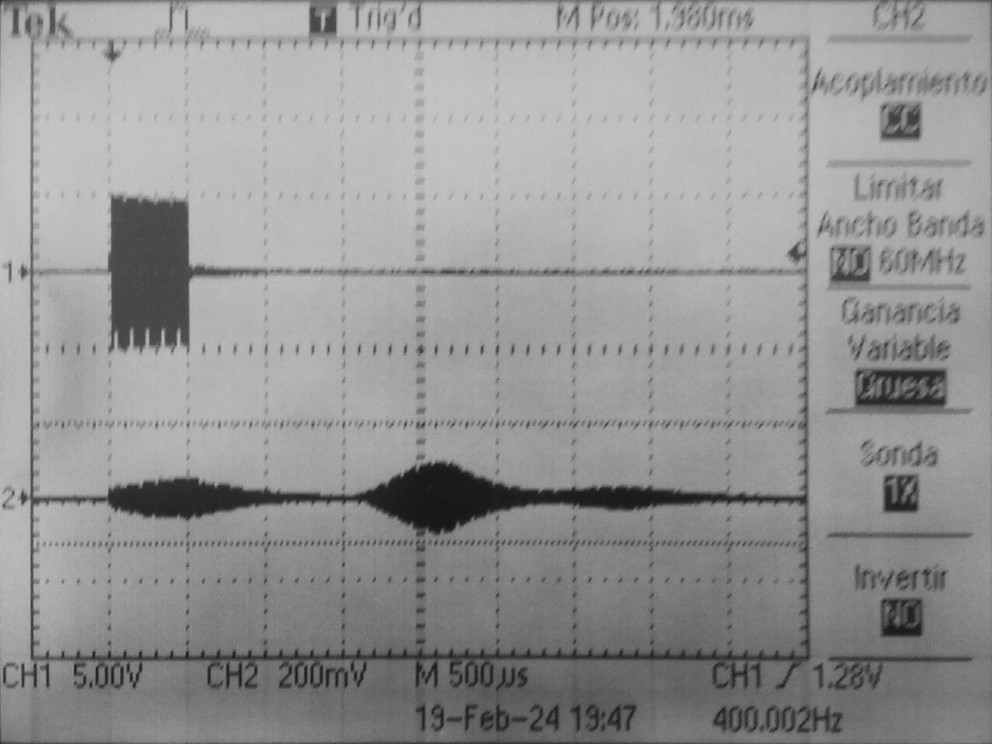
\includegraphics[width=295px]{1_1.png}
  \end{center}
  \caption{Recepció del pols sense amplificador}
  \label{fig:1_1}
\end{figure}

\newthought{Qüestió L1.2: } S'ha posat un obstacle a \qty{25}{\centi\meter}, $TOF\simeq\qty{1.5}{\milli\second}$ que implica una distància mesurada de $\simeq\qty{25}{\centi\meter}$. L'amplitud màxima és de uns \qty{200}{\milli\volt}.

\newthought{Qüestió L1.3: } Igual que la figura \ref{fig:1_1} pero l'amplitud màxima és de \qty{12}{\volt}, la saturació del AO.

\newthought{Qüestió L1.4: } Veure la figura \ref{fig:1_4}. S'ha fet la mesura apuntant al sostre.

\begin{figure}
  \begin{center}
    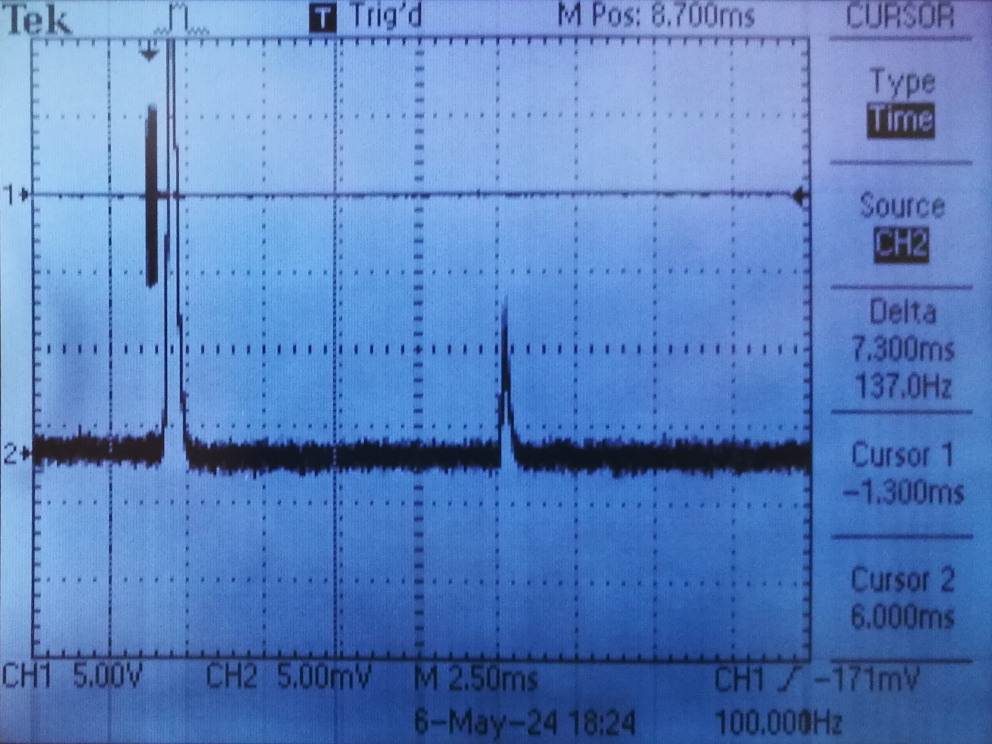
\includegraphics[width=295px]{1_4.png}
  \end{center}
  \caption{Sortida del detector d'envolupant apuntant al sostre}
  \label{fig:1_4}
\end{figure}

\newthought{Qüestió L1.5: } El TOF és de $\simeq\qty{11.25}{\milli\second}$. La distància del sostre fins al damunt del ordinador (el punt de mesura) és de $\simeq\qty{1.9}{\meter}$.

\newthought{Qüestió L1.6: } Veure la figura \ref{fig:1_6}.

\begin{figure}
  \begin{center}
    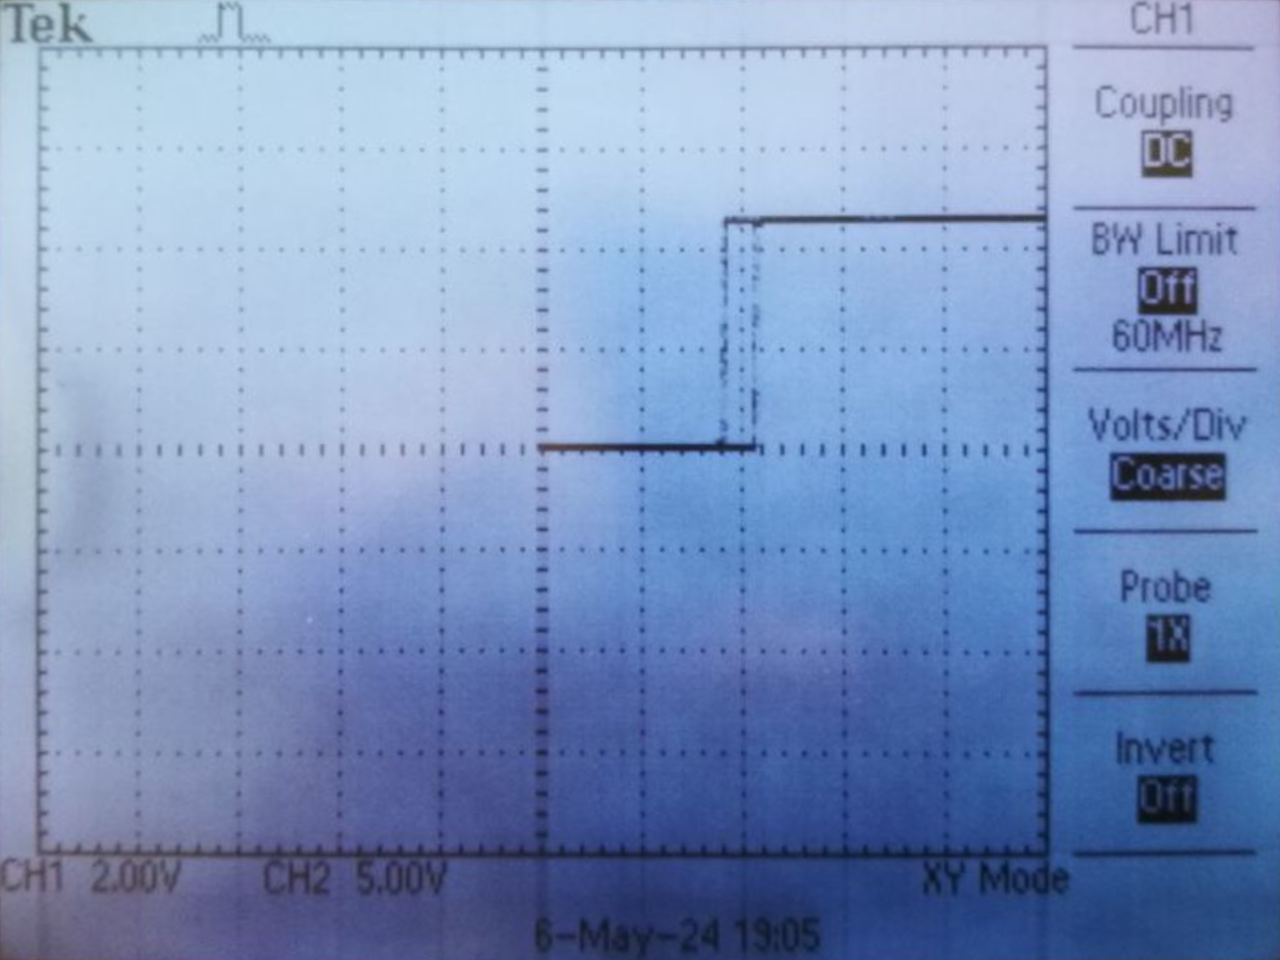
\includegraphics[width=295px]{1_6.png}
  \end{center}
  \caption{Resposta entrada-sortida del comparador amb histèresi}
  \label{fig:1_6}
\end{figure}

\newthought{Qüestió L1.7: } Canvia el nivell de tensió al que es provoca un canvi de tensió a la sortida. El cicle de histèresi però, es mantè constant.

\newthought{Qüestió L1.9: } Veure la figura \ref{fig:1_9}.

\begin{figure}
  \begin{center}
    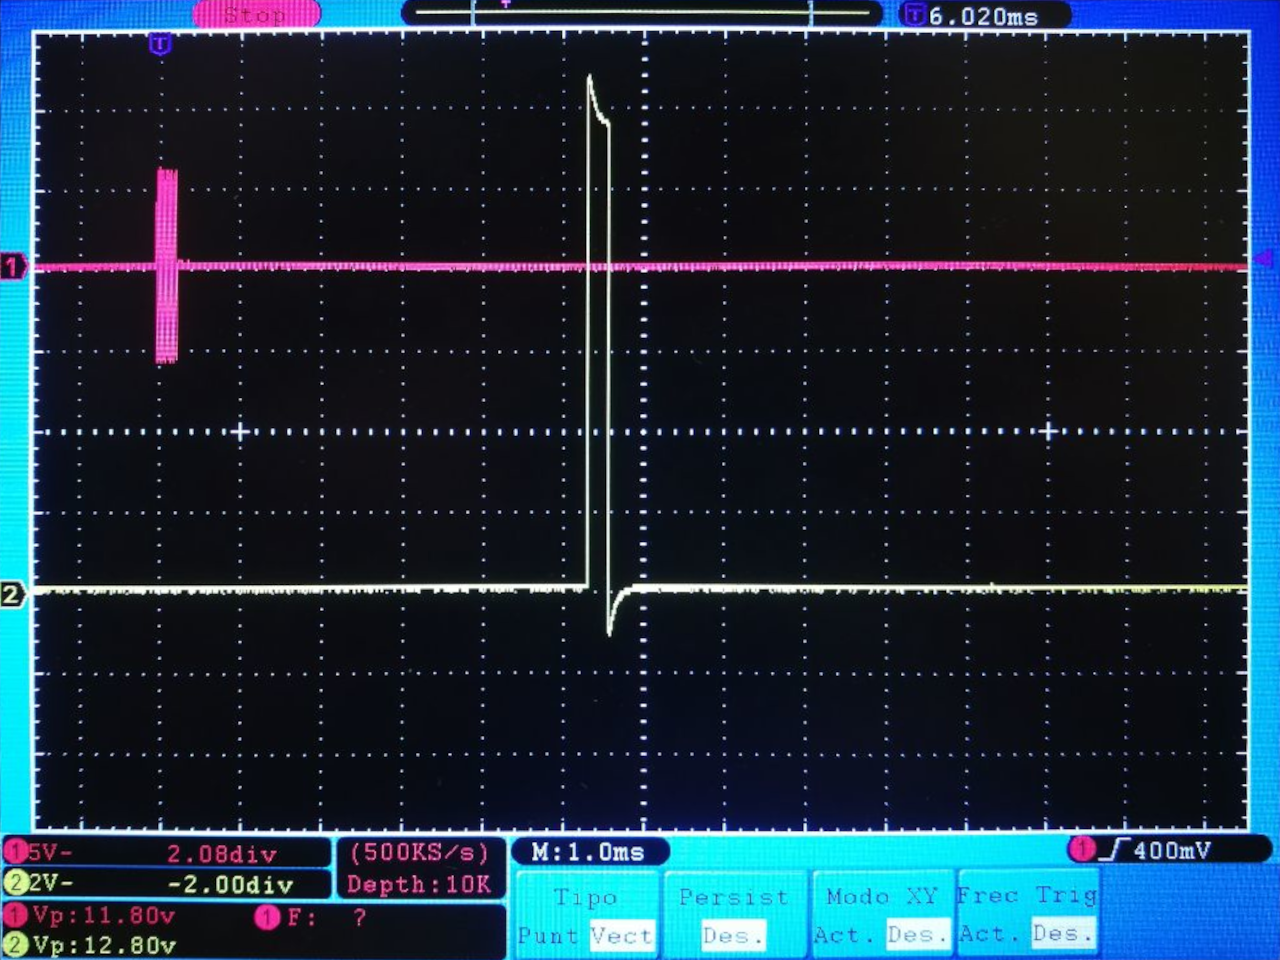
\includegraphics[width=295px]{1_9.png}
  \end{center}
  \caption{Sortida del detector de nivell}
  \label{fig:1_9}
\end{figure}

\newthought{Qüestió L1.10} S'estava mesurant la paret. $TOF\simeq\qty{5.5}{\milli\second}$ implica una distància de $\simeq\qty{1}{\meter}$.

\part{Segona sessió}

\newthought{Qüestió L2.1: } Variant el potenciòmetre s'obtenen freqüencies de \qty{25}{\kilo\hertz} fins a \qty{55}{\kilo\hertz}.

\newthought{Qüestió L2.2: } Veure la figura \ref{fig:2_2}. Freqüència de \qty{40}{\kilo\hertz} i $V_{pp} = \qty{12}{\volt}$.

\begin{figure}
  \begin{center}
    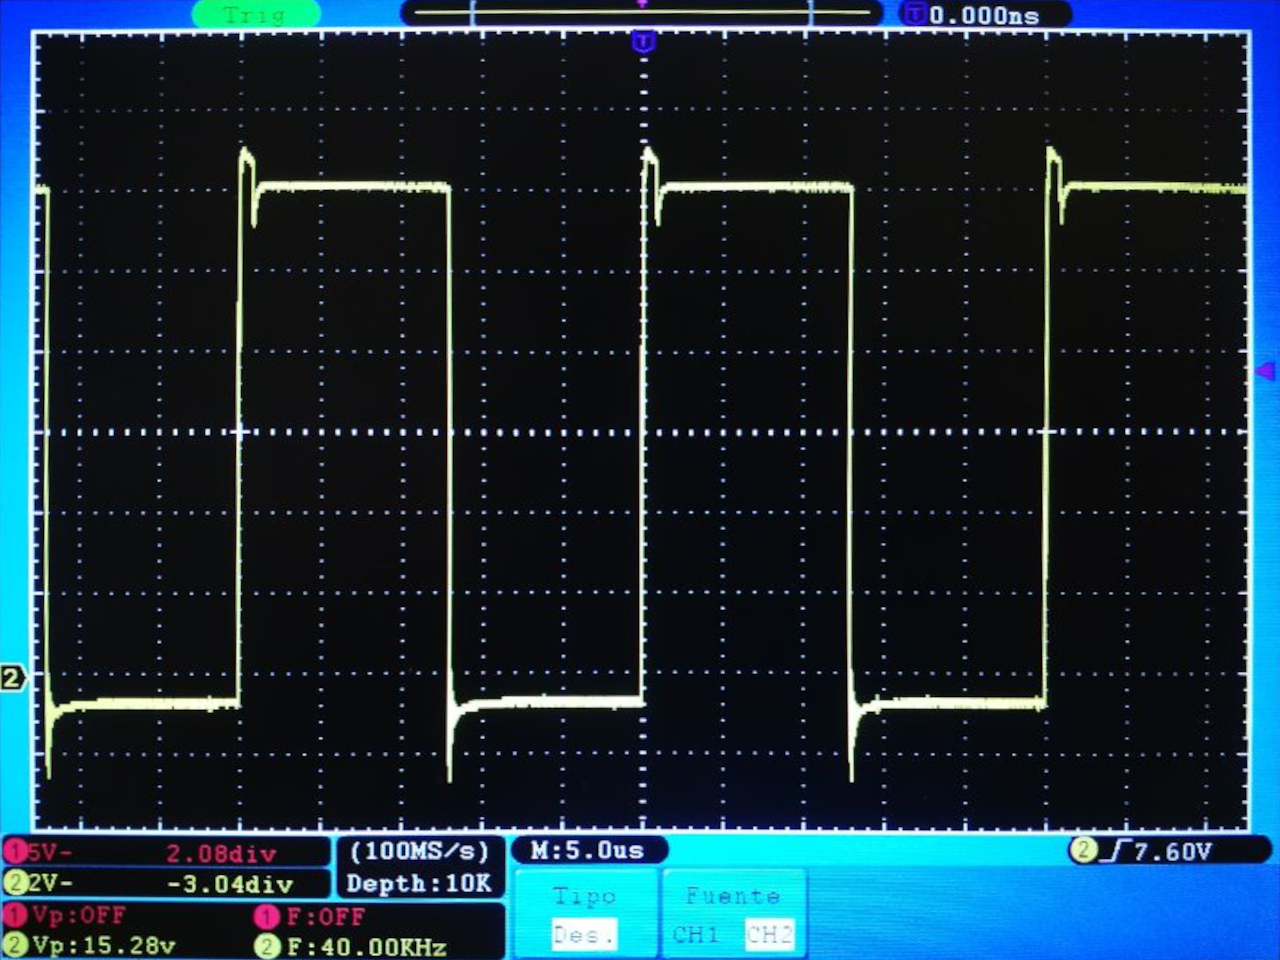
\includegraphics[width=295px]{2_2.png}
  \end{center}
  \caption{Sortida del generador d'ona cuadrada}
  \label{fig:2_2}
\end{figure}

\newthought{Qüestió L2.3: } Configurat a \qty{40}{\kilo\hertz} el cicle de treball és $\simeq\qty{50}{\percent}$.

\newthought{Qüestió L2.4: } A la meitat del recorregut la duració del pol val \qty{1}{\milli\second}.

\newthought{Qüestió L2.5: } La durada del pols haurà de ser $\frac{10}{f}=\qty{250}{\micro\second}$. La repetició \qty{30}{\hertz}.

\newthought{Qüestió L2.6: } Veure les figures \ref{fig:2_6_1} i \ref{fig:2_6_2}. Hi ha \num{11} cicles per salva, la salva es repeteix amb una freqüència de \qty{29.7}{\hertz}, i la freqüència del senyal de la salva val \qty{39.9}{\kilo\hertz}. S'han de fer ajustaments.

\begin{figure}
  \begin{center}
    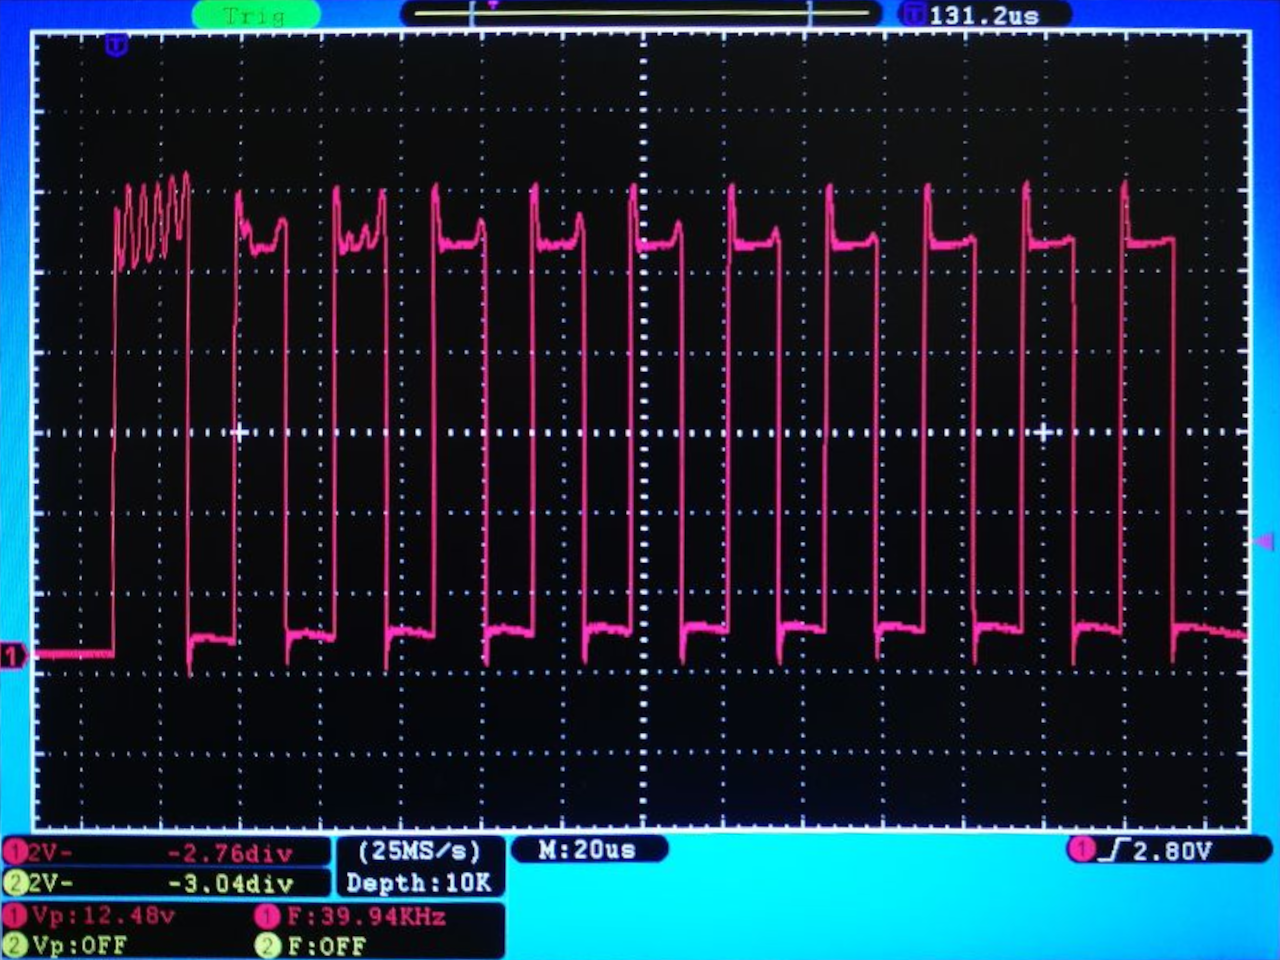
\includegraphics[width=295px]{2_6_1.png}
  \end{center}
  \caption{Cicles per salva}
  \label{fig:2_6_1}
\end{figure}

\begin{figure}
  \begin{center}
    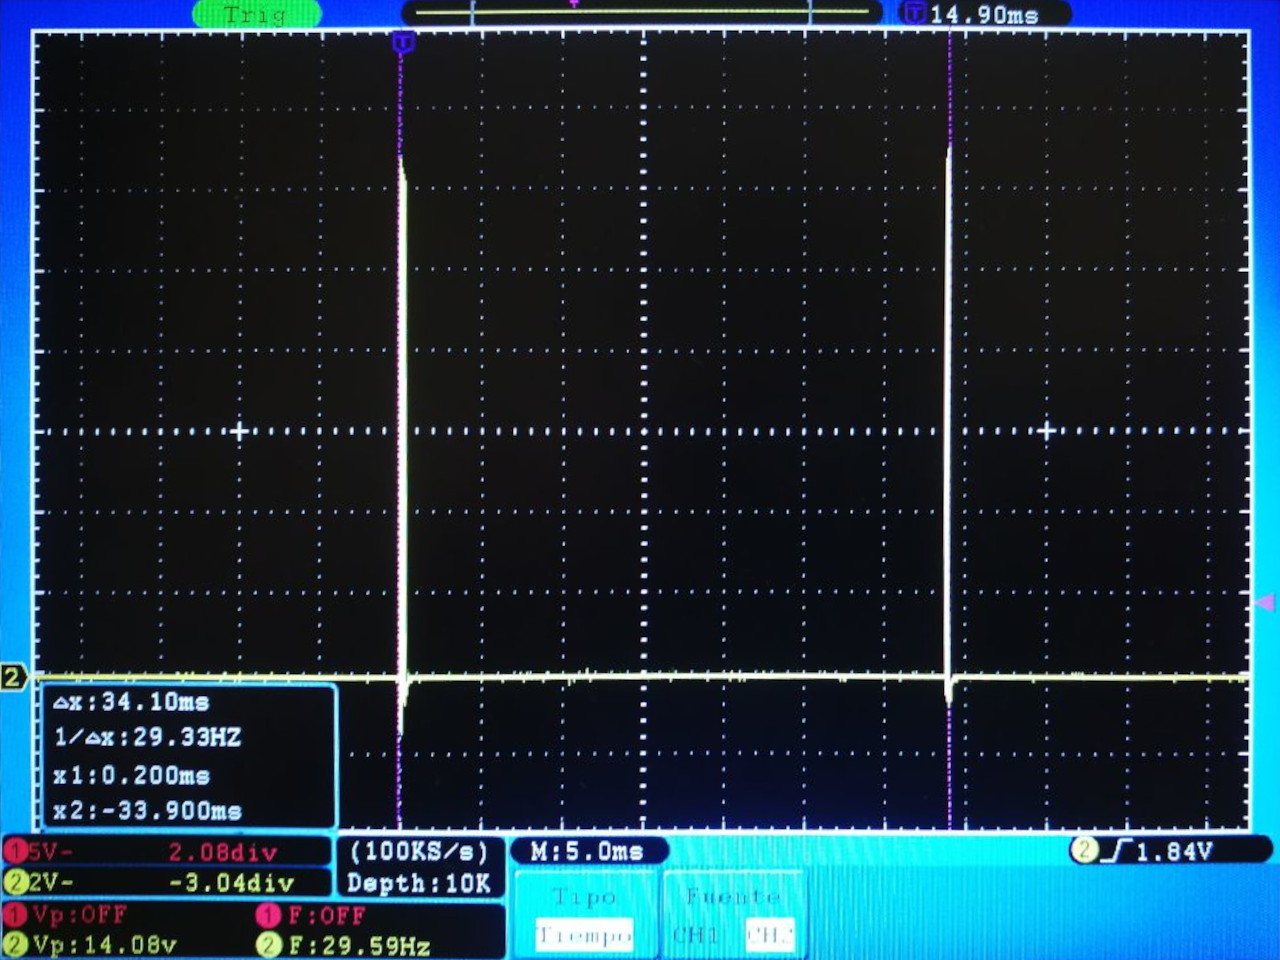
\includegraphics[width=295px]{2_6_2.png}
  \end{center}
  \caption{Repetició de salves}
  \label{fig:2_6_2}
\end{figure}

\newthought{Qüestió L2.7: } Veure la figura \ref{fig:2_7}.

\begin{figure}
  \begin{center}
    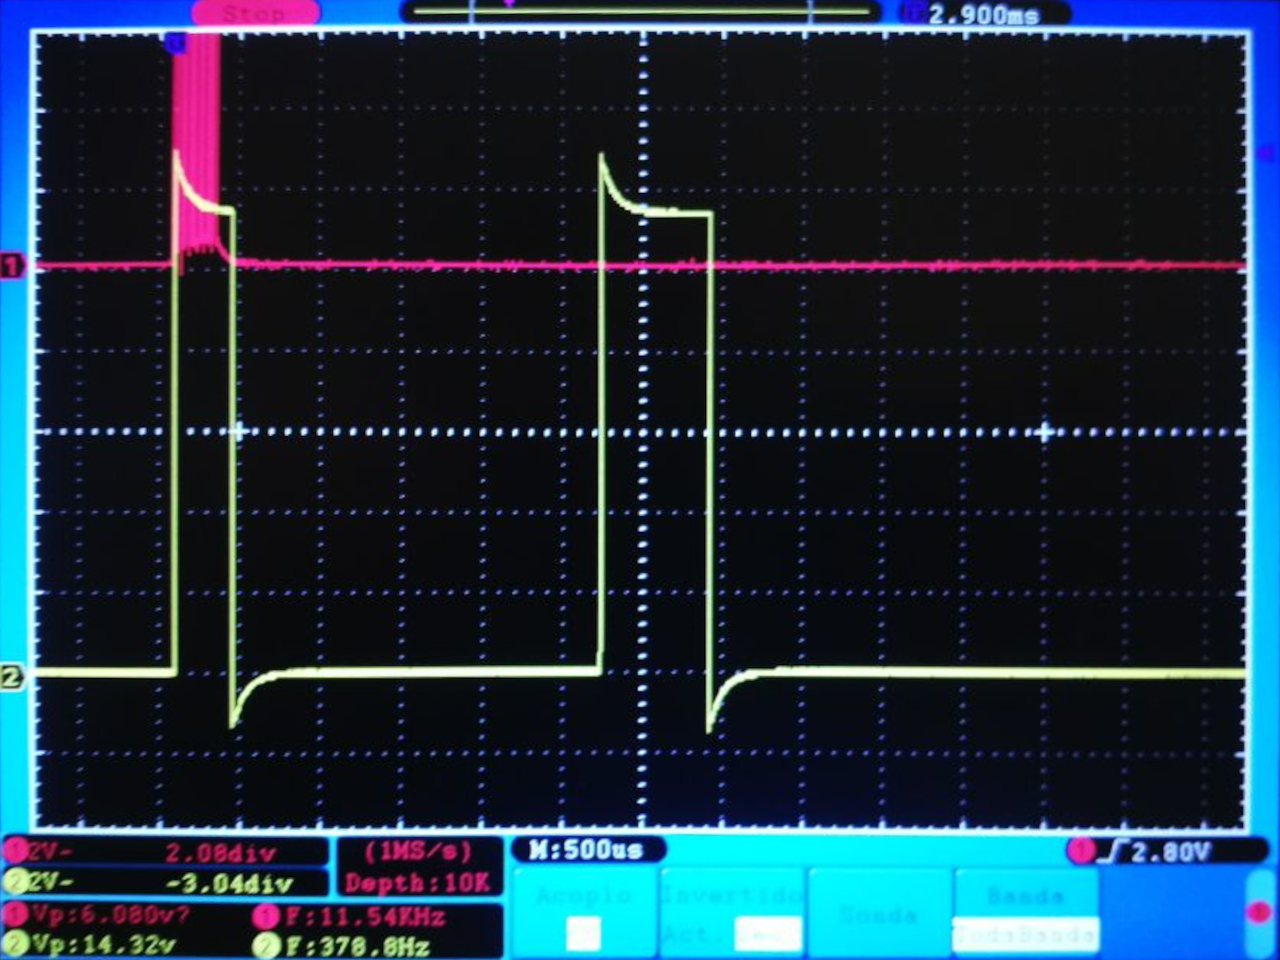
\includegraphics[width=295px]{2_7.png}
  \end{center}
  \caption{Prova de funcionament de la salva}
  \label{fig:2_7}
\end{figure}

\part{Tercera sessió}

\newthought{Qüestió L3.1: } La freqüència pot variar entre els \qty{10.7}{\kilo\hertz} i els \qty{19.6}{\kilo\hertz}.

\newthought{Qüestió L3.2: } Veure la figura \ref{fig:3_2}. El senyal té un $V_{pp}$ de casi \qty{13}{\volt}.

\begin{figure}
  \begin{center}
    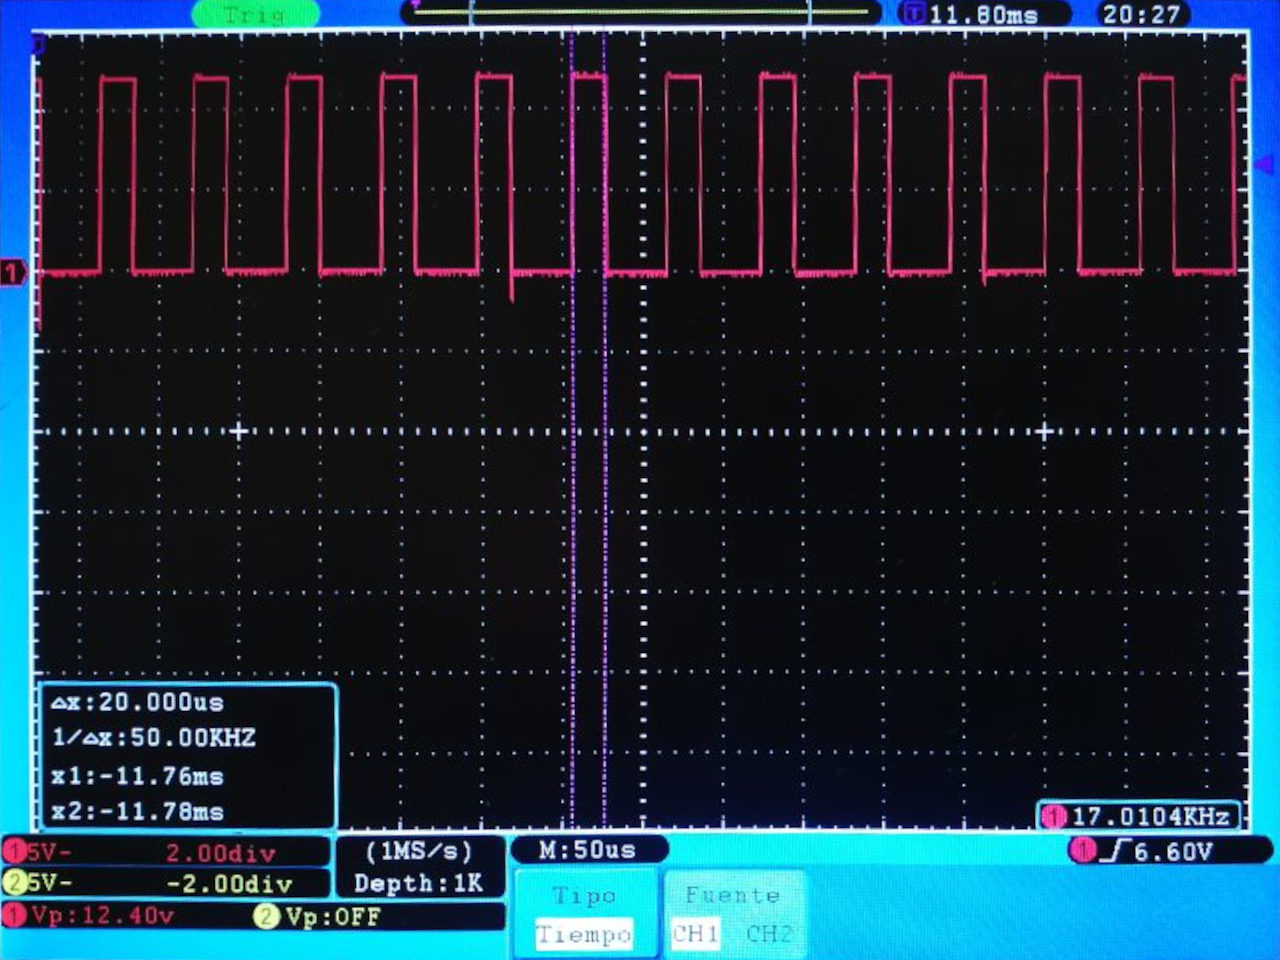
\includegraphics[width=295px]{3_2.png}
  \end{center}
  \caption{Senyal clock}
  \label{fig:3_2}
\end{figure}

\newthought{Qüestió L3.3: } Està en valor alt \qty{20}{\micro\second} i el periode val \qty{50}{\micro\second}. Per tant el cicle de treball és del \qty{34}{\percent}.

\newthought{Qüestió L3.4: } Veure la figura \ref{fig:3_4}. El display mostra $050$ per al muntatge sencer.

\begin{figure}
  \begin{center}
    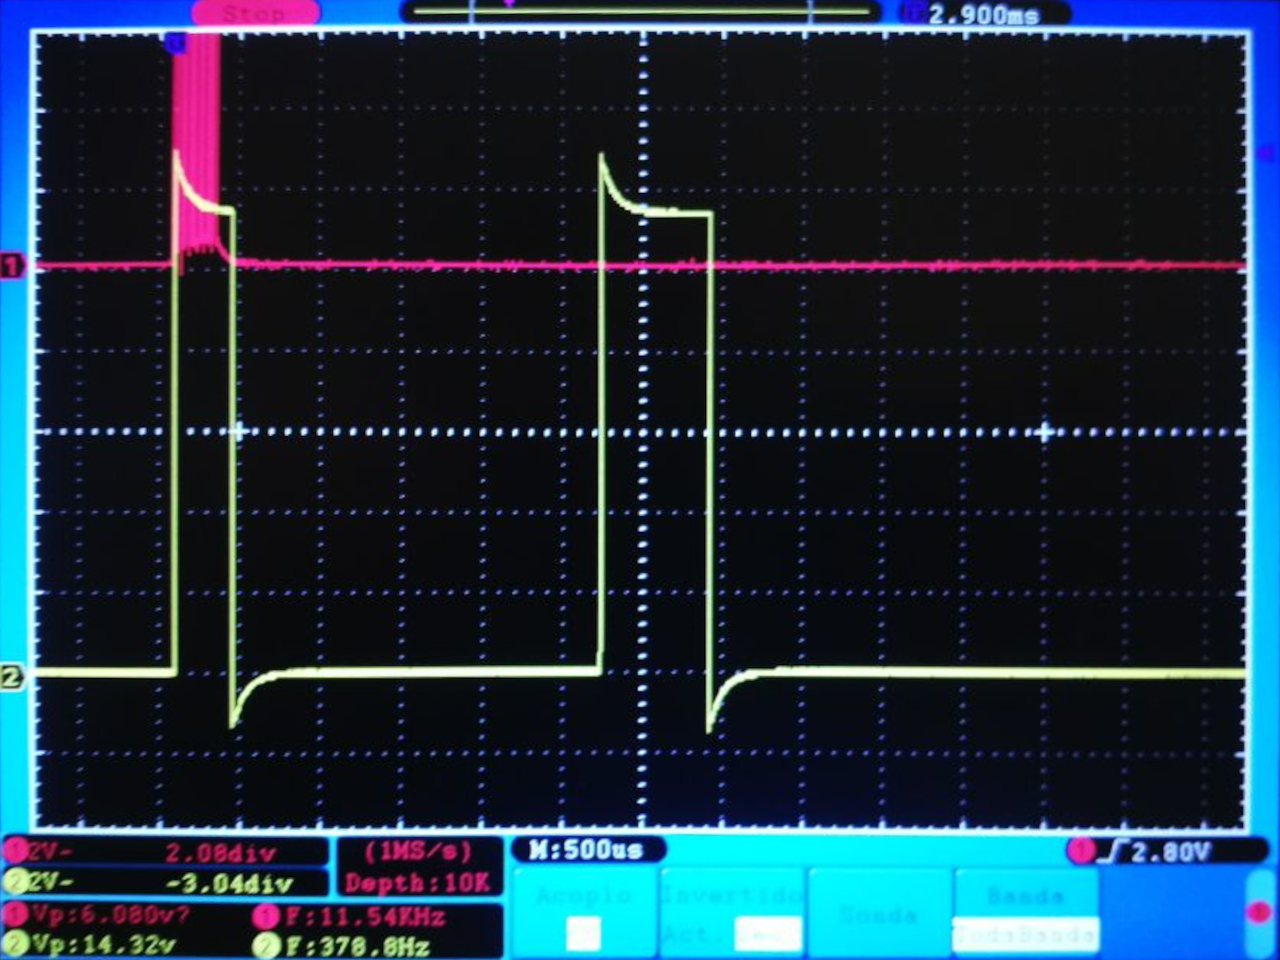
\includegraphics[width=295px]{3_4.png}
  \end{center}
  \caption{Demostració del conjunt amb un obstacle a \qty{0.5}{\meter}}
  \label{fig:3_4}
\end{figure}

\newthought{Qüestió L3.5: } Com es pot observar a la figura \ref{fig:3_5}, el nostre mesurador arriba fins als \qty{2.56}{\meter}.

\begin{figure}
  \begin{center}
    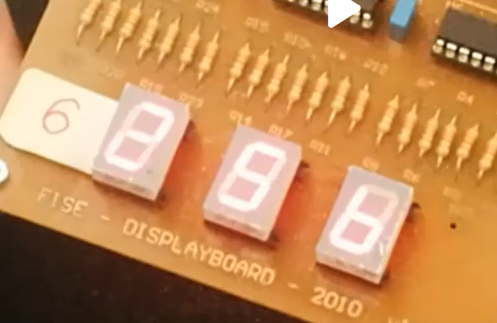
\includegraphics[width=295px]{3_5.png}
  \end{center}
  \caption{Mesura a màxima distància}
  \label{fig:3_5}
\end{figure}

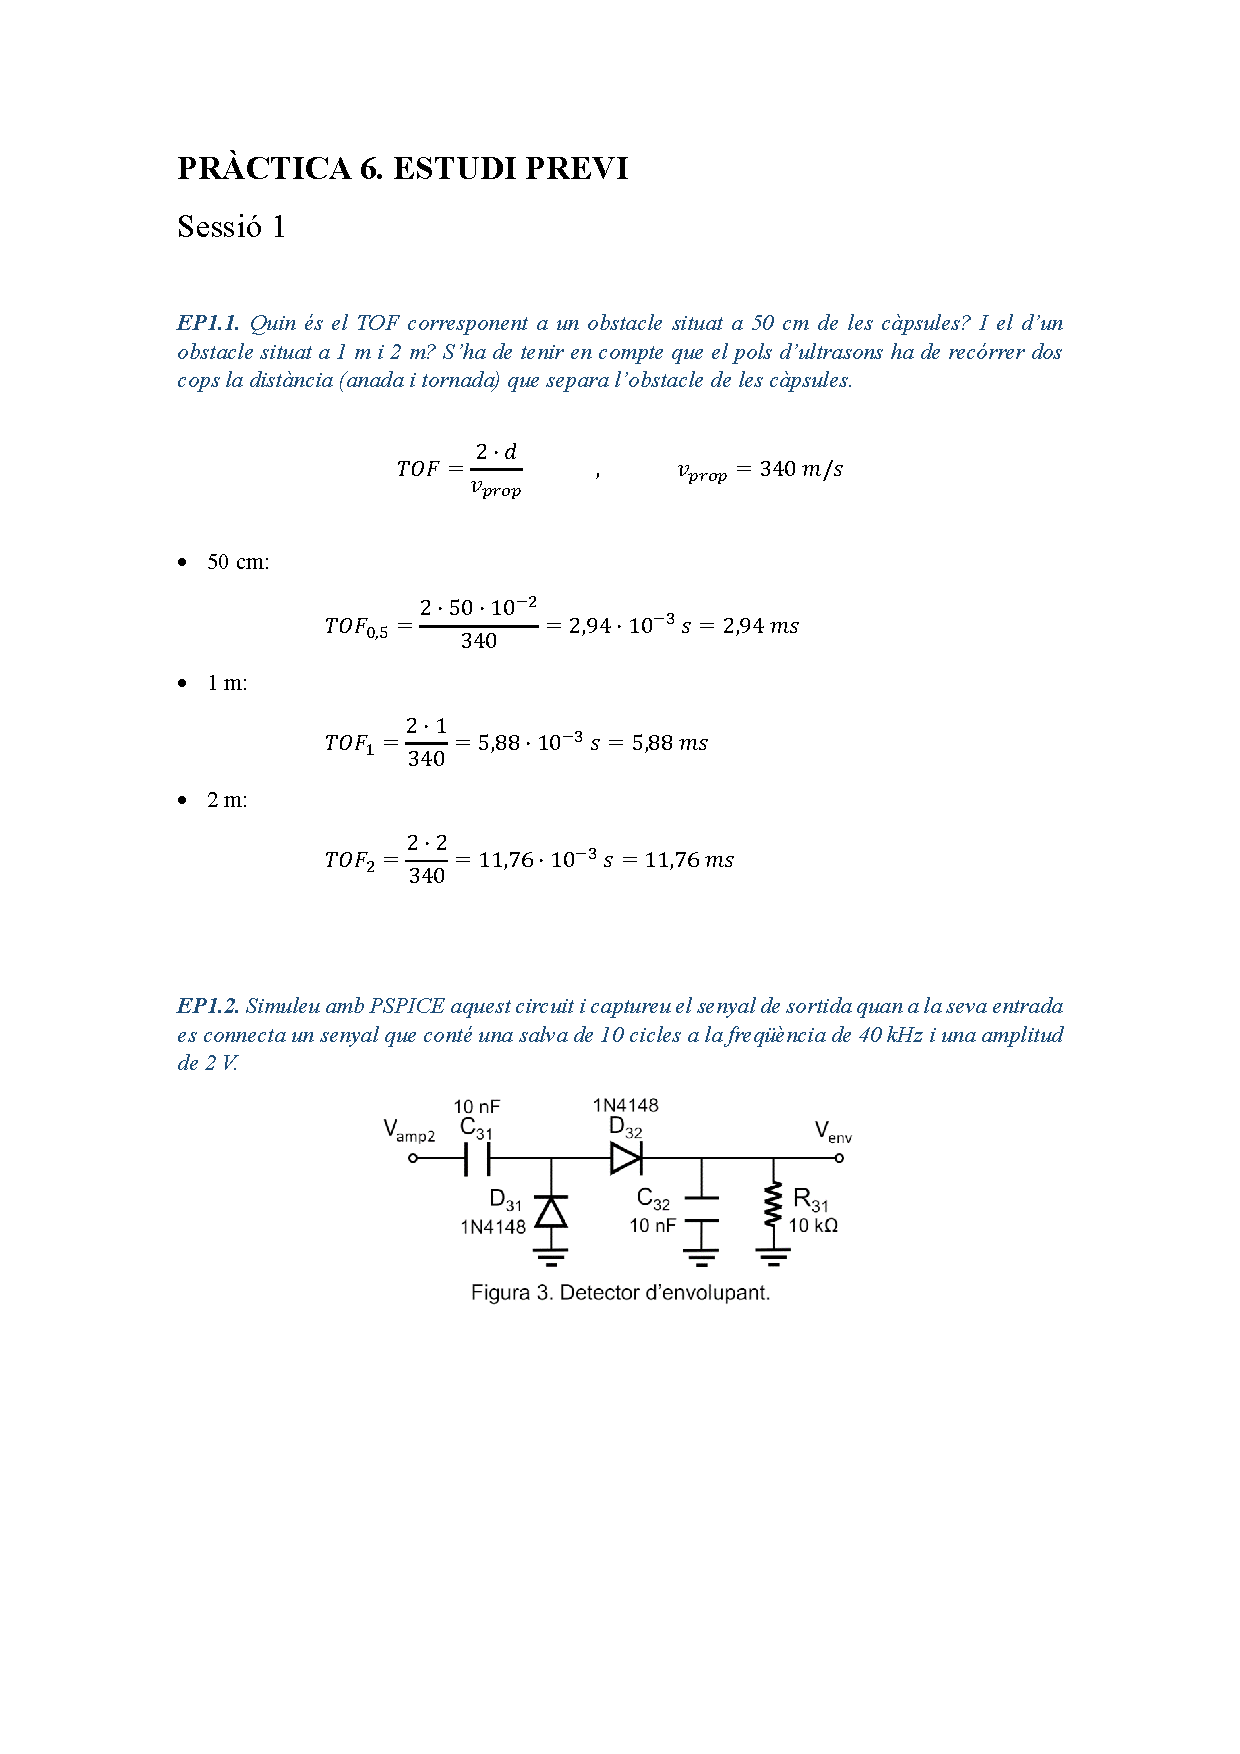
\includepdf[pages={1-7}]{P6_estudi_previ.pdf}

\end{document}